
\section{Overview}
Swarm robotics focus on the coordination of multiple robots trying to reach a certain goal. In most scenarios, this involves limited communication abilities between robots and the restriction to local information. Although control is decentralized, as each robot is autonomous, emergent behavior can be observed, enabling the swarm to solve problems that a single robot can't.

\subsection{The Swarm Bot}
Here, the relevant artifact is called \emph{Swarm Bot}. It consists of several mobile \emph{S-Bots}, who can connect to and disconnect from each other.
\begin{figure}\centering
\includegraphics[width=0.8\textwidth]{pics/sbots2.jpg}
\caption{A swarm of six S-Bots, five of them connected}
\end{figure}
The Swarm Bot can be used for various tasks, including moving objects and moving through tough physical terrain. Furthermore, due to the ability to disconnect one or more S-Bots from itself, it can use them for tasks like finding a goal or tracing an optimal path, where single S-Bots may be more efficient.\\
In this paper we will focus on two tasks: \emph{Aggregation} and \emph{coordinated motion}. Aggregation describes the ability of several scattered S-Bots to minimize the distance between each other. Coordinated motion represents the ability of a connected Swarm Bot to move in a single direction. Both tasks are considered mandatory for the development of more complex behavior.

\subsection{Self organization}
As mentioned before, in most scenarios swarm robots are limited to local information. Therefore, it is important to apply mechanisms that can deal with this restriction while still being able to show emergent behavior.\\
\emph{Self organization} describes such mechanisms for biological systems, but can also be applied to swarm robotics. The System state depends on positive and negative feedback:\\
\emph{Positive feedback} represents the amplification of a certain property emerging from random interactions. It increases exponentially over time.\\
\emph{Negative feedback} works as a regulation which is triggered by positive feedback exhausting some resource. By the interaction of positive and negative feedback, the system is kept in a stable state. \cite[pp. 11--20]{camazine2003self}\\
The difficulty in creating self organizing Systems is the fact, that the relation between individual and global behavior is hard to analyze: Given a set of individual behaviors, it is difficult to predict the
behavior that is going to emerge on a system level. On the other hand, given global behavior, it is difficult to decompose individual behaviors leading to it.

\subsection{Artificial evolution}
A possible solution for this problem is \emph{artificial evolution}. It can be used to generate individual behavior, while evaluating the system as a whole and therefore bypassing the derivation of individual rules from global behavior. For the Swarm Bot, we will use artificial evolution to create controllers for each S-Bot. The controllers are realized through artificial neural networks, connecting sensory input to motor output. A genetic algorithm then determines optimal weight matrices for these networks.\\
Artificial evolution is based on the biological equivalent. It optimizes individuals on the basis of a given \emph{fitness function}, using \emph{selection}, \emph{reproduction} and \emph{mutation}. \cite[pp. 37--69]{eiben03genetic}\\
The general process of a genetic algorithm is as follows:
\begin{enumerate}
	\item An initial population is created randomly
	\item The fitness of all individuals in the current population is evaluated by applying the fitness function
	\item A subset of well-fit individuals is selected for reproduction
	\item Offspring is created and altered using mutation
	\item Steps 2--4 are repeated until a certain stop criterion (e.g. fitness threshold, timeout) is met
\end{enumerate}
Note that recombination is not used here, as it doesn't perform well for evolving weight matrices of neural networks. \cite[pp. 1425--1428]{yao1999evolving}


\subsection{Artificial neural networks}
As mentioned above, an artificial neural network is used to connect sensory input to motor output. Like genetic Algorithms, artificial neural networks are inspired by biology. There is a vast variety of different types of neural networks. Here, the relevant network architecture is the \emph{single layer perceptron}.

\begin{figure}\centering
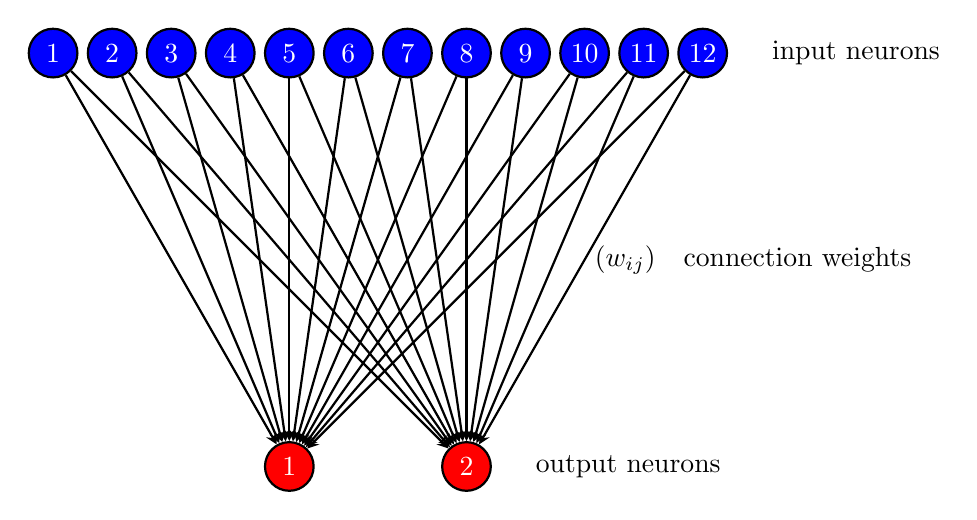
\begin{tikzpicture}[thick, scale=.75]
\node[circle, draw, fill=red, text=white] (O1) at (5, 0) {1};
\node[circle, draw, fill=red, text=white] (O2) at (8, 0) {2};
\foreach \i in {1, 2, ..., 12} {
	\node[circle, draw, fill=blue, label={center:\color{white}\i}] (I\i) at (\i, 7) {\phantom{0}};
	\draw[->, >=stealth] (I\i) -> (O1);
	\draw[->, >=stealth] (I\i) -> (O2);
}
\node[right] at (13,7) {input neurons};
\node[right] at (10, 3.5) {$\left( w_{ij} \right)$};
\node[right] at (11.5, 3.5) {connection weights};
\node[right] at (9,0) {output neurons};
\end{tikzpicture}
\caption{A single layer perceptron with 12 input neurons and two output neurons}
\end{figure}
The Neurons are arranged in two layers, one input and one output layer. Each input neuron is connected to each output neuron. All neural connections are \emph{weighted}.
A neuron's weighted input is mapped to its output using a given \emph{activation function}. Here, a \emph{sigmoid function} will be used:
\begin{figure}[h]\centering
\begin{tikzpicture}[domain=-2.2:2.2, smooth, samples=50, >=stealth, scale=2, thick]

\draw[color=blue] plot (\x,{1 / (1+exp(- 4 *\x))}) node at (2.5, 0.7) {};

% Koordinatenachsen
\draw[->] (-2.2,0) -- (2.2,0) node[right] {$x$};
\draw[->] (0,-0.2) -- (0,1.2) node[above] {$f(x) = \dfrac{1}{1+e^{-ax}}$};
\draw (-0.05,1) --(0.05,1) node [left] {$1~$};
\draw (-0.05,0.5) -- (0.05,0.5) node [left] {$0.5~$};
\foreach \i in {-2, -1, 1, 2}{
	\draw (\i, -0.05) -- (\i, 0.05) node [below=1ex] {$\i$};
}
\end{tikzpicture}
\caption{The sigmoid function used in the experiment}\label{sigmoid}
\end{figure}
\newpage
The functionality of the network depends on the following parameters:
\begin{enumerate}
	\item Network topology, i.e. number of layers and neurons per layer
	\item The activation function
	\item Connection weights.
\end{enumerate}
In the following experiment, the S-Bot controllers only differ in (3).




